% (The MIT License)
%
% Copyright (c) 2023-2025 Yegor Bugayenko
%
% Permission is hereby granted, free of charge, to any person obtaining a copy
% of this software and associated documentation files (the 'Software'), to deal
% in the Software without restriction, including without limitation the rights
% to use, copy, modify, merge, publish, distribute, sublicense, and/or sell
% copies of the Software, and to permit persons to whom the Software is
% furnished to do so, subject to the following conditions:
%
% The above copyright notice and this permission notice shall be included in all
% copies or substantial portions of the Software.
%
% THE SOFTWARE IS PROVIDED 'AS IS', WITHOUT WARRANTY OF ANY KIND, EXPRESS OR
% IMPLIED, INCLUDING BUT NOT LIMITED TO THE WARRANTIES OF MERCHANTABILITY,
% FITNESS FOR A PARTICULAR PURPOSE AND NONINFRINGEMENT. IN NO EVENT SHALL THE
% AUTHORS OR COPYRIGHT HOLDERS BE LIABLE FOR ANY CLAIM, DAMAGES OR OTHER
% LIABILITY, WHETHER IN AN ACTION OF CONTRACT, TORT OR OTHERWISE, ARISING FROM,
% OUT OF OR IN CONNECTION WITH THE SOFTWARE OR THE USE OR OTHER DEALINGS IN THE
% SOFTWARE.

\documentclass{article}
\usepackage{../lecture-notes/notes}
\usepackage{svg}
\newcommand*\thetitle{Cognitive Complexity}
\begin{document}

\lnTitlePage{3}{24}{oRUux3w4rsc}

\lnThought{Cyclomatic complexity is highly inaccurate if being compared with code readability evaluated by a human.}

\lnQuote
  [Bill Curtis]
  {bill-curtis}
  {Computational complexity assesses the difficulty of verifying an algorithm's correctness, while psychological complexity assesses human performance on programming tasks.}
  {curtis1979measuring}

\lnQuote
  [Lionel C. Briand]
  {lionel-briand}
  {By cognitive complexity we mean the \ul{mental burden} of the persons who have to deal with the class. We \ul{assume} that it is the, sometimes necessary, high cognitive complexity of a class which causes it to display undesirable external qualities, such as decreased maintainability and testability, or increased fault-proneness.}
  {briand2001integrating}

\lnQuote
  [Jingqiu Shao]
  {jingqiu-shao}
  {Cognitive complexity, the \ul{new measure} for software complexity presented in this paper, is a measure of the cognitive and psychological complexity of software as a human intelligence artifact.}
  {shao2003new}

\lnPitch{
  \begin{multicols}{2}
  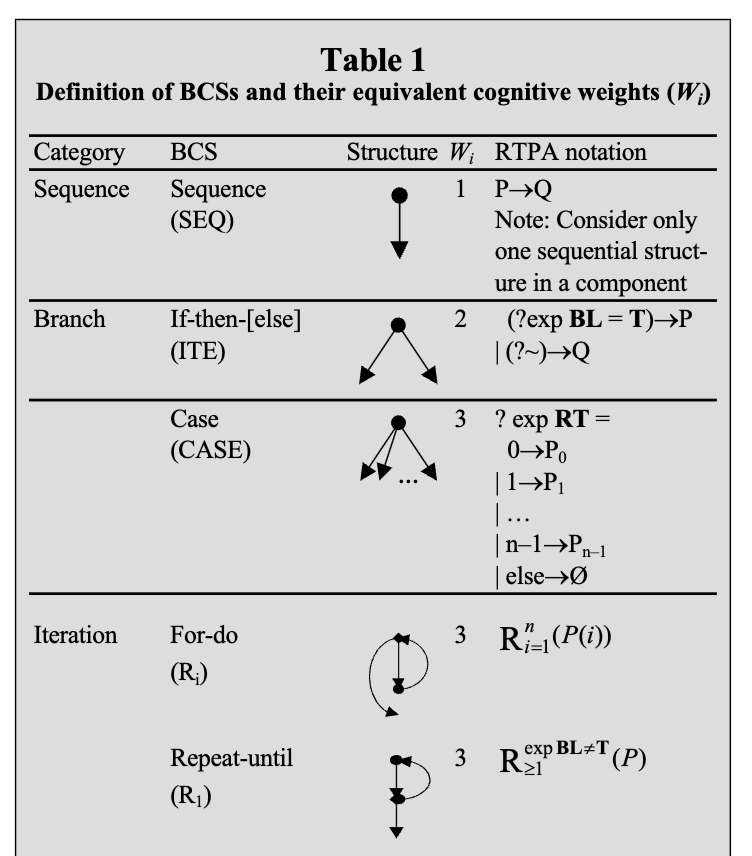
\includegraphics[width=.8\linewidth]{bcs.png}\par
  BCS stands for ``\ul{basic control structure}.''
  \par\columnbreak\par
  ``The cognitive weight of software is the degree of difficulty or relative time and effort required for comprehending a given piece of software modelled by a number of BCSs. The total cognitive weight of a software component, \(W_c\), is defined as the sum of the cognitive weights of its \(q\) linear blocks composed of individual BCSs.''
  \par
  \lnSource{shao2003new}
  \end{multicols}}

\lnQuote
  {yingxu-wang}
  {Cognitive complexity of software is a product of its architectural and operational complexities on the basis of \ul{deductive semantics} and the \ul{abstract system theory}.}
  {wang2006cognitive}

\lnQuote
  [Dharmender Singh Kushwaha]
  {dharmender-singh-kushwaha}
  {We developed an improved cognitive information complexity measure (CICM) that is based on the amount of information contained in the software and encompasses all the major parameters that have a bearing on the difficulty of comprehension or cognitive complexity of software.}
  {kushwaha2006improved}

\lnPitch{
  \begin{multicols}{2}
  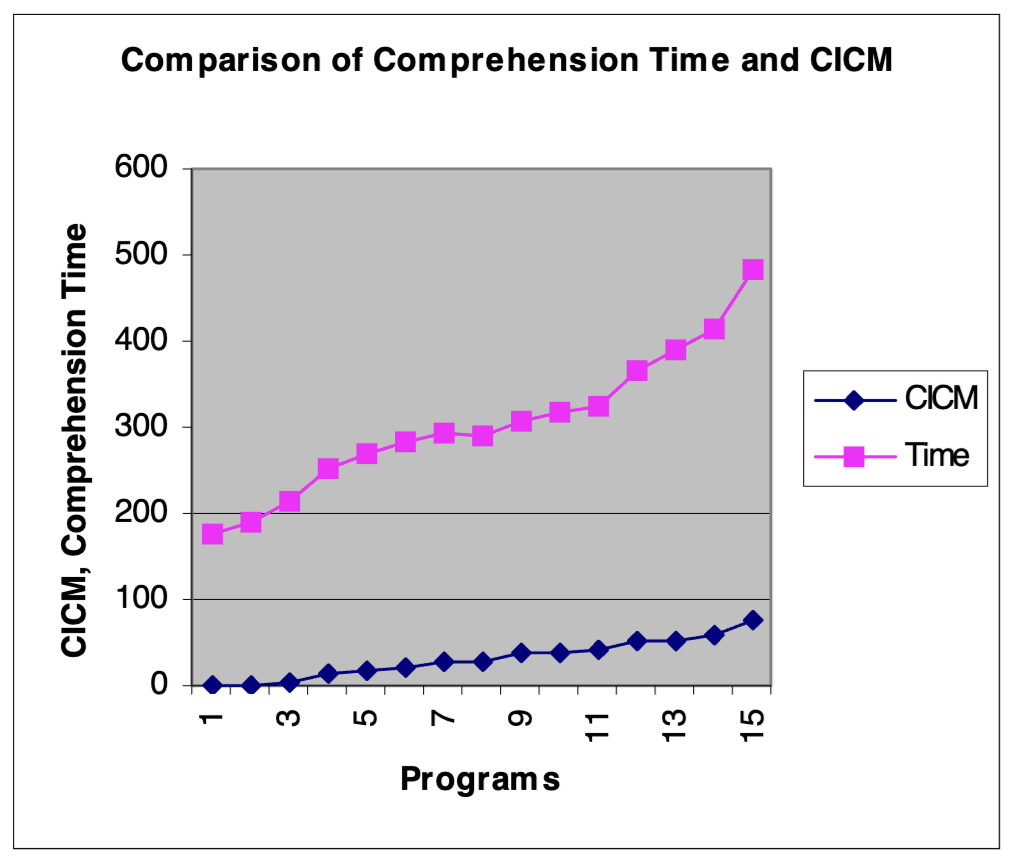
\includegraphics[width=.95\linewidth]{cicm.png}\par
  \par\columnbreak\par
  ``In a group of 25, each student was given 15 programs. They were asked to read the program and come out with what problem the program addressed. Time required to understand was recorded. The diagram shows that as cognitive information complexity increases, time taken to understand the program also increased.''
  \par
  \lnSource{kushwaha2006improved}
  \end{multicols}}

\lnQuote
  {anonymous}
  {The cognitive weight of a BCS is measured as the number of ways that BCS can generate some factors that make it difficult to comprehend relative to the sequential BCS, of which the cognitive weight is `1'. The value of total cognitive weights of the software is measured as the number of relative ways that software can generate the combination of factors that make the function and semantics difficult to comprehend.}
  {benjapol2008underlying}

\lnQuote
  [Ann Campbell]
  {ann-campbell}
  {A guiding principle in the formulation of Cognitive Complexity has been that it should incent \ul{good} coding practices. That is, it should either ignore or discount features that make code more readable.\pptPin{
\includegraphics[width=7em]{sonarqube.pdf}}}
  {campbell2018cognitive}

\lnPitch{
  \pptPic{.9}{motive-before.png}\par
  ``The mathematical model underlying \ul{Cyclomatic Complexity} gives these two
  methods equal weight, yet it is intuitively obvious that the control flow of
  \ff{sumOfPrimes} is more difficult to understand than that of \ff{getWords}.''
  \lnSource{campbell2017}}

\lnPitch{
  \pptPic{.9}{motive-after.png}\par
  ``The \ul{Cognitive Complexity} algorithm gives these two methods markedly different
  scores, ones that are far more reflective of their relative understandability.''
  \lnSource{campbell2017}}

\lnQuote
  [Rub{\'e}n Saborido]
  {ruben-saborido}
  {Different cognitive complexity measures have been proposed to quantify the understandability of a piece of code and, therefore, its maintainability. \ul{However}, the cognitive complexity metric provided by SonarSource is quickly spreading in the software industry due to the popularity of their well-known static code \ul{tools} for evaluating software quality.}
  {saborido2022automatizing}

\lnPitch{Cognitive Complexity (\textcolor{orange}{CoCo}) is supported by a few static analyzers:
  \begin{itemize}
  \setlength\itemsep{0em}
  \item for Java by PMD \href{https://pmd.github.io/pmd/pmd_rules_apex_design.html}{since 6.22.0}
  \item for Ruby by Rubocop \href{https://www.rubydoc.info/gems/rubocop/RuboCop/Cop/Metrics/PerceivedComplexity}{since 0.25} (called ``perceived complexity'')
  \item for C++ by \href{https://docs.codeclimate.com/docs/cognitive-complexity}{CodeClimate}
  \item for JavaScript by ESLint via \href{https://github.com/SonarSource/eslint-plugin-sonarjs/blob/master/docs/rules/cognitive-complexity.md}{SonarSource plugin}
  \item for Python by Flake8 via \href{https://github.com/Melevir/flake8-cognitive-complexity}{this plugin}
  \item for Rust by Clippy \href{https://rust-lang.github.io/rust-clippy/master/\#/cognitive_complexity}{since 1.35.0}
  \item for PHP by PHPCS via \href{https://github.com/Rarst/phpcs-cognitive-complexity}{this plugin}
  \end{itemize}}

\lnThought{Maybe it's impossible to accurately measure the ``\ul{perceived} complexity'' of software?}

\lnQuote
  {norman-fenton}
  {We showed that the search for \ul{general} software complexity measures is doomed to failure.}
  {fenton1994software}

\lnQuote
  [Luigi Lavazza]
  {luigi-lavazza}
  {Being able to find statistical correlations between code \ul{understandability} and source code \ul{measures} would be greatly beneficial for the software development process, which involves a great deal of activities involving program \ul{comprehension}.}
  {lavazza2023empirical}

\lnThought{Social code analysis: we analyze the \ul{author(s)} of the code, not only the code itself.}

\lnQuote
  {../03-cognitive-complexity/social}
  {Social code analysis enriches our understanding of the code quality by overlaying a \ul{developer's behavior} with the \ul{structural analysis} of the code.}
  {social2017}

\lnPitch{
  \pptQuote{helmet.jpg}{BrainMaster Technologies (USA) sells this ``\href{https://brainmaster.com/product/freedom-20r-series/}{Freedom 20R}'' EEG head set for \$31,025. A similar device you can get from \href{https://neiry.ru/about-us}{Neiry} (Russia), for 3\% of this price.}{}}

\lnQuote
  {raul-barbosa}
  {We propose the use of \ul{biofeedback} code highlighting techniques to provide online programmer's warnings for potentially problematic code lines that may need a second look at (to remove possible bugs).}
  {couceiro2019spotting}

The following Java code has an obvious but hard to spot functional defect:
\par
{\scriptsize\begin{ffcode}[columns=flexible]
public class AverageCalculator {                             // (*@\textcolor{green}{LOW}@*)
  public static void main(String[] args) {                   // (*@\textcolor{green}{LOW}@*)
    int[] numbers = {10, 20, 30, 40, 50};                    // (*@\textcolor{green}{LOW}@*)
    System.out.println("Average: " + avg(numbers));          // (*@\textcolor{orange}{MEDIUM}@*)
  }                                                          // (*@\textcolor{green}{LOW}@*)
  static double avg(int[] nums) {                            // (*@\textcolor{green}{LOW}@*)
    double sum = 0;                                          // (*@\textcolor{orange}{MEDIUM}@*)
    for (int i = 0; i (*@\textcolor{red}{<=}@*) nums.length; i++)                   // (*@\textcolor{red}{HIGH}@*)
      sum += nums[i];                                        // (*@\textcolor{red}{HIGH}@*)
    return sum / nums.length;                                // (*@\textcolor{orange}{MEDIUM}@*)
  }                                                          // (*@\textcolor{green}{LOW}@*)
}                                                            // (*@\textcolor{green}{LOW}@*)
\end{ffcode}
}
\par
The ``cognitive state code annotations'' are on the right side of the code, as Java comments, indicating the level of \ul{brain activity} at the moment of writing the particular line of code.
\plush{}

\lnQuote
  {julio-medeiros}
  {The EEG results reveal evidence of \ul{mental effort saturation} as \ul{code complexity} increases. Conversely, the classic software complexity metrics do \ul{not accurately} represent the mental effort involved in code comprehension.}
  {medeiros2021can}

\end{document}
